\section{Vejledermøde 6}

\vspace{0.5 cm}
\textbf{Indkaldelse til vejledermøde \#6} \\

Dato: 8-11-2018 \\
Tid: 12:00 \\
Sted: 408E \\
Deltagere: () Til stede, (F) for sent, (A) meldt afbud, (U) Udeblev \\
Caroline(), Kajene(), Mathias(), Mikkel(), Nicolai(), Sarah(), Thea(F), Samuel() 

\vspace{0.1 cm}
\textbf{Dagsorden:}

\begin{enumerate}
	\item Valg af mødeleder
	\item Valg af referent
	\item Godkendelse af referat fra forrige møde
	\item Opfølgning af aktionspunkter fra forrige møde
	\item Spørgsmål til Samuel
	\item Gennemgang af tidsplan
	\item Nye aktionspunkter til næste møde
	\item Tidspunkt for næste møde
	\item Evt.
\end{enumerate}

\textbf{Referat:}

\begin{enumerate}
	\item Mathias
	\item Nicolai
	\item Godkendt
	\item Aktionspunkter: Bruger Pivotal Tracker
	\item \textbf{Forlænger til transducer:} \\
	Finder 4 ledninger og erstatter dem med en han/hun ved at klipse dem sammen. \\
	\textbf{Physiobank:} \\
	Find signal for 10 sekunder og gå længere ind i målingen, hvor der sker noget i signalet. \\
	\textbf{Valgt på forhånd hvilke tryk, der kalibreres med?} \\
	Vi skal kalibrere ved følgende tryk: 10, 50 og 100. Vil være en god idé at tage 30 og 75 med i kalibreringen. - Vær opmærksom på interpolation. Vi må ikke tillade os at sige at den måler korrekt, da vi ikke kan teste helt op til vores max tryk på 250 mmhg.
	\textbf{Hvornår skal alarm afspilles igen?} \\
	Der skal gå mellem 2.5 s og 15.0 s før alarmen spilles igen. Kig i standarderne som ses nedenfor:
	
	\begin{figure}[h!]
		\centering
		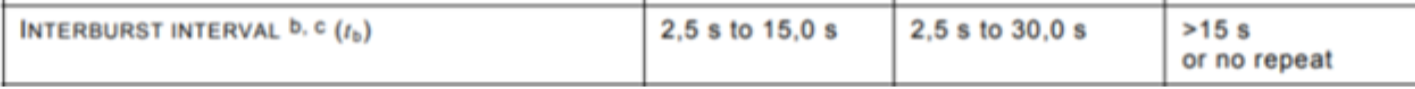
\includegraphics[width=1\linewidth]{Vejledermoeder/Standard}
	\end{figure}
	
	\item Godkendt
	\item Find tidspunkt til udførelse af accepttest
	\item Næste møde: 25-10-2018 kl. 12:00 
	\item Deadline på bestilling af print: 2 uger
	
\end{enumerate}

\clearpage